
% vim: set ft=tex tabstop=4 shiftwidth=4 noexpandtab:

% opening %{{{1

\documentclass[tikz, border=1mm]{standalone}

% packages and libraries %{{{1

% ---- not necessary since the documentclass[tikz ...] requires it automatically
% \usepackage{tikz}

\usetikzlibrary{calc,intersections,angles,quotes,shapes.geometric}

\usepackage{amsmath}

\usepackage{tkz-euclide}


\begin{document}
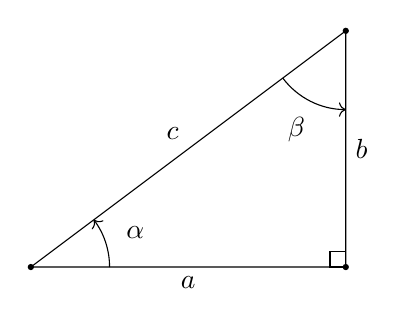
\begin{tikzpicture}[scale=1.0]

	\coordinate (A) at (0,0);
	\coordinate (B) at (4,0);
	\coordinate (C) at (4,3);

	\draw (A) -- (B) -- (C) -- cycle;

	\fill (A) circle (0.4mm);
	\fill (B) circle (0.4mm);
	\fill (C) circle (0.4mm);

	\node[below] at ($(A)!0.5!(B)$) {$a$};
	\node[above left]  at ($(A)!0.5!(C)$) {$c$};
	\node[right] at ($(B)!0.5!(C)$) {$b$};

	\pic["$\alpha$", draw, ->, angle eccentricity=1.4, angle radius=1.0cm]
		{angle = B--A--C};
	\pic["$\beta$", draw, ->, angle eccentricity=1.4, angle radius=1.0cm]
		{angle = A--C--B};

	\tkzMarkRightAngle[size=0.2](C,B,A)

\end{tikzpicture}
\end{document}
